\documentclass[]{article}
\usepackage{lmodern}
\usepackage{amssymb,amsmath}
\usepackage{ifxetex,ifluatex}
\usepackage{fixltx2e} % provides \textsubscript
\ifnum 0\ifxetex 1\fi\ifluatex 1\fi=0 % if pdftex
  \usepackage[T1]{fontenc}
  \usepackage[utf8]{inputenc}
\else % if luatex or xelatex
  \ifxetex
    \usepackage{mathspec}
  \else
    \usepackage{fontspec}
  \fi
  \defaultfontfeatures{Ligatures=TeX,Scale=MatchLowercase}
\fi
% use upquote if available, for straight quotes in verbatim environments
\IfFileExists{upquote.sty}{\usepackage{upquote}}{}
% use microtype if available
\IfFileExists{microtype.sty}{%
\usepackage{microtype}
\UseMicrotypeSet[protrusion]{basicmath} % disable protrusion for tt fonts
}{}
\usepackage[margin=1in]{geometry}
\usepackage{hyperref}
\hypersetup{unicode=true,
            pdftitle={Laborator 5},
            pdfborder={0 0 0},
            breaklinks=true}
\urlstyle{same}  % don't use monospace font for urls
\usepackage{graphicx,grffile}
\makeatletter
\def\maxwidth{\ifdim\Gin@nat@width>\linewidth\linewidth\else\Gin@nat@width\fi}
\def\maxheight{\ifdim\Gin@nat@height>\textheight\textheight\else\Gin@nat@height\fi}
\makeatother
% Scale images if necessary, so that they will not overflow the page
% margins by default, and it is still possible to overwrite the defaults
% using explicit options in \includegraphics[width, height, ...]{}
\setkeys{Gin}{width=\maxwidth,height=\maxheight,keepaspectratio}
\IfFileExists{parskip.sty}{%
\usepackage{parskip}
}{% else
\setlength{\parindent}{0pt}
\setlength{\parskip}{6pt plus 2pt minus 1pt}
}
\setlength{\emergencystretch}{3em}  % prevent overfull lines
\providecommand{\tightlist}{%
  \setlength{\itemsep}{0pt}\setlength{\parskip}{0pt}}
\setcounter{secnumdepth}{5}
% Redefines (sub)paragraphs to behave more like sections
\ifx\paragraph\undefined\else
\let\oldparagraph\paragraph
\renewcommand{\paragraph}[1]{\oldparagraph{#1}\mbox{}}
\fi
\ifx\subparagraph\undefined\else
\let\oldsubparagraph\subparagraph
\renewcommand{\subparagraph}[1]{\oldsubparagraph{#1}\mbox{}}
\fi

%%% Use protect on footnotes to avoid problems with footnotes in titles
\let\rmarkdownfootnote\footnote%
\def\footnote{\protect\rmarkdownfootnote}

%%% Change title format to be more compact
\usepackage{titling}

% Create subtitle command for use in maketitle
\newcommand{\subtitle}[1]{
  \posttitle{
    \begin{center}\large#1\end{center}
    }
}

\setlength{\droptitle}{-2em}

  \title{Laborator 5}
    \pretitle{\vspace{\droptitle}\centering\huge}
  \posttitle{\par}
  \subtitle{Funcția de repartiție și cuantilele empirice}
  \author{}
    \preauthor{}\postauthor{}
    \date{}
    \predate{}\postdate{}
  
\usepackage{booktabs}
\usepackage{longtable}
\usepackage{framed,color}
\definecolor{shadecolor}{RGB}{248, 248, 248}
\definecolor{shadecolor1}{RGB}{216,225,235}
\definecolor{framecolor}{RGB}{16,111,124}%108,123,13

%\definecolor{shadecolor}{RGB}{226, 255, 241}
% \definecolor{shadecolor1}{RGB}{217,225,199}
% \definecolor{framecolor}{RGB}{60,179,113}

%%%%%%%%%%%%%%%%%%%%%%
\ifxetex
  \usepackage{letltxmacro}
  \setlength{\XeTeXLinkMargin}{1pt}
  \LetLtxMacro\SavedIncludeGraphics\includegraphics
  \def\includegraphics#1#{% #1 catches optional stuff (star/opt. arg.)
    \IncludeGraphicsAux{#1}%
  }%
  \newcommand*{\IncludeGraphicsAux}[2]{%
    \XeTeXLinkBox{%
      \SavedIncludeGraphics#1{#2}%
    }%
  }%
\fi

\newenvironment{frshaded*}{%
  \def\FrameCommand{\fboxrule=\FrameRule\fboxsep=\FrameSep \fcolorbox{framecolor}{shadecolor1}}%
  \MakeFramed {\advance\hsize-\width \FrameRestore}}%
{\endMakeFramed}

\newenvironment{rmdblock}[1]
  {\begin{frshaded*}
  \begin{itemize}
  \renewcommand{\labelitemi}{
    \raisebox{-.7\height}[0pt][0pt]{
      {\setkeys{Gin}{width=2em,keepaspectratio}\includegraphics{images/icons/#1}}
    }
  }
  \item
  }
  {
  \end{itemize}
  \end{frshaded*}
  }
  
%%%%%%%%%%%%%%%
% definitions.
% -------------------
\usepackage{marginnote}
% \renewcommand*{\marginnotevadjust}{40pt}
% \renewcommand{\marginnotevadjust}{0pt}
% \renewcommand{\marginfont}{\noindent\rule{0pt}{0.7\baselineskip}\tiny}

\newtheorem{proposition}{Proposition}[section]
\newtheorem{lemma}[proposition]{Lemma}
\newtheorem{corollary}[proposition]{Corollary}
\newtheorem{theorem}[proposition]{Theorem}

\newcounter{exo}[section]
\newcommand{\enonce}[2]{\refstepcounter{proposition}\hypertarget{exo:#1}{}\label{exo:#1}{\scriptsize\;\textbf{Ex.}~\ref{exo:#1}}}

\reversemarginpar
\setlength{\marginparwidth}{1.2cm}
% 
% \newcommand{\enonce}[2]{\refstepcounter{proposition}\hypertarget{exo:#1}{}\label{exo:#1}{\noindent\color{black}\normalsize\bf Exercice \ref{exo:#1}}\ \  #2\vspace{1mm}\hrule\vspace{1mm} \color{black}\normalsize}


%%%%%%%%%%%%%%%

% \newenvironment{rmdcaution}
%   {\begin{rmdblock}{caution}}
%   {\end{rmdblock}}

% \newenvironment{rmdinsight}
%   {\begin{rmdblock}{insight}}
%   {\end{rmdblock}}

\newenvironment{rmdexercise}
  {\begin{rmdblock}{exercise}}
  {\end{rmdblock}}

% \newenvironment{rmdexercise_tex}
%   {\begin{rmdblock}{exercise}}
%   {\end{rmdblock}}
  
% \newenvironment{rmdtip}
%   {\begin{rmdblock}{tip}}
%   {\end{rmdblock}}


%%%%%%%%%%%%%%%%%%%%%%%%%%%%%%%%%%%%%%%%%%%%%%%%%%%%%%%%%%%%%%%%%%%%%%%%%%%%%%%%%%%%%%%%%%%%%%%%%%%%%%%%%%%%%%%%%%%%%
%%%%%%%%%%% For insight block %%%%%%%%%%%%%%%%%%%%%%%%%%
\definecolor{shadecolor_insight}{RGB}{223,240,216}
\definecolor{framecolor_insight}{RGB}{136,193,137}

%\definecolor{shadecolor_insight}{RGB}{217,225,199}
%\definecolor{framecolor_insight}{RGB}{60,179,113}

\newenvironment{frshaded_insight*}{%
  \def\FrameCommand{\fboxrule=\FrameRule\fboxsep=\FrameSep \fcolorbox{framecolor_insight}{shadecolor_insight}}%
  \MakeFramed {\advance\hsize-\width \FrameRestore}}%
{\endMakeFramed}

\newenvironment{rmdblock_insight}[1]
  {\begin{frshaded_insight*}
  \begin{itemize}
  \renewcommand{\labelitemi}{
    \raisebox{-.7\height}[0pt][0pt]{
      {\setkeys{Gin}{width=2em,keepaspectratio}\includegraphics{images/icons/#1}}
    }
  }
  \item
  }
  {
  \end{itemize}
  \end{frshaded_insight*}
  }

\newenvironment{rmdinsight}
  {\begin{rmdblock_insight}{insight}}
  {\end{rmdblock_insight}}

%%%%%%%%%%% For caution block %%%%%%%%%%%%%%%%%%%%%%%%%%
\definecolor{shadecolor_caution}{RGB}{250,250,250}
\definecolor{framecolor_caution}{RGB}{242,129,67}%193,75,34

\newenvironment{frshaded_caution*}{%
  \def\FrameCommand{\fboxrule=\FrameRule\fboxsep=\FrameSep \fcolorbox{framecolor_caution}{shadecolor_caution}}%
  \MakeFramed {\advance\hsize-\width \FrameRestore}}%
{\endMakeFramed}

\newenvironment{rmdblock_caution}[1]
  {\begin{frshaded_caution*}
  \begin{itemize}
  \renewcommand{\labelitemi}{
    \raisebox{-.7\height}[0pt][0pt]{
      {\setkeys{Gin}{width=2em,keepaspectratio}\includegraphics{images/icons/#1}}
    }
  }
  \item
  }
  {
  \end{itemize}
  \end{frshaded_caution*}
  }
  
\newenvironment{rmdcaution}
  {\begin{rmdblock_caution}{caution}}
  {\end{rmdblock_caution}}

%%%%%%%%%%% For tip block %%%%%%%%%%%%%%%%%%%%%%%%%%
\definecolor{shadecolor_tip}{RGB}{250,250,250}
\definecolor{framecolor_tip}{RGB}{33,153,195}

\newenvironment{frshaded_tip*}{%
  \def\FrameCommand{\fboxrule=\FrameRule\fboxsep=\FrameSep \fcolorbox{framecolor_tip}{shadecolor_tip}}%
  \MakeFramed {\advance\hsize-\width \FrameRestore}}%
{\endMakeFramed}

\newenvironment{rmdblock_tip}[1]
  {\begin{frshaded_tip*}
  \begin{itemize}
  \renewcommand{\labelitemi}{
    \raisebox{-.7\height}[0pt][0pt]{
      {\setkeys{Gin}{width=2em,keepaspectratio}\includegraphics{images/icons/#1}}
    }
  }
  \item
  }
  {
  \end{itemize}
  \end{frshaded_tip*}
  }
  
\newenvironment{rmdtip}
  {\begin{rmdblock_tip}{tip}}
  {\end{rmdblock_tip}}

%%%%%%%%%%%%%%%%%%%%%%%%%%%%%%%%%%%%%%%%%%%%%%%%%%%%%%%%%%%%%%%%%%%%%%%%%%%%%%%%%%%%%%%%%%%%%%%%%%%%%%%%%%%%%%%%%%%%%
\usepackage{subfigure}
\usepackage{booktabs}
\usepackage{slashbox}
\usepackage{color}
%%%%%%%%%%%%%%%%%%%%%%%%%%%%%%%%%%%%%%%%%
\definecolor{linkcol}{rgb}{0,0,0.4}
\definecolor{citecol}{rgb}{0.5,0,0}

% Change this to change the informations included in the pdf file
% \usepackage[pagebackref]{hyperref}
% \usepackage[verbose]{backref}
\usepackage[hyperpageref]{backref}
% \backrefsetup{verbose=false}
% \PassOptionsToPackage{pagebackref}{hyperref}
% See hyperref documentation for information on those parameters

\hypersetup
{
bookmarksopen=true,
pdftitle="Curs Statistica",
pdfauthor="Alexandru Amarioarei",
pdfsubject="Curs Statistica", %subject of the document
pdfmenubar=true, %menubar shown
pdfhighlight=/O, %effect of clicking on a link
colorlinks=true, %couleurs sur les liens hypertextes
pdfpagemode=None, %aucun mode de page
pdfpagelayout=SinglePage, %ouverture en simple page
pdffitwindow=true, %pages ouvertes entierement dans toute la fenetre
linkcolor=linkcol, %couleur des liens hypertextes internes
citecolor=citecol, %couleur des liens pour les citations
urlcolor=linkcol %couleur des liens pour les url
}


% set the back references
\renewcommand*{\backref}[1]{}
\renewcommand*{\backreftwosep}{ și~} % inserted between entries 
                              % in a list of two entries, 
                              % default is " and~".
\renewcommand*{\backreflastsep}{ și~} % inserted between the last 
                               % two entries of a list with more
                               % than two entries, default is ", and~".
\renewcommand*{\backrefalt}[4]{%
    \ifcase #1 (Necitat.)%
    \or        (Citat la pagina~#2.)%
    \else      (Citat la paginile~#2.)%
    \fi}

%%%%%%%%%%%%%%%%%%%%%%%%%%%%%%%%%%%%%%%%%%%%%%%%%%%%%%%%%%%%%%%%%%%%%%%%%%%%%%%%%%%%%%%%%%%%%%%%%%%%%%%%%%%%%%%%%%%%%
%CITEVA DEFINITII
\def\om{\omega}
\def\Om{\Omega}
\def\et{\eta}
\def\td{\tilde{\delta}}
\def\m{{\mu}}
\def\n{{\nu}}
\def\k{{\kappa}}
\def\l{{\lambda}}
\def\L{{\Lambda}}
\def\g{{\gamma}}
\def\a{{\alpha}}
\def\e{{\varepsilon}}
\def\b{{\beta}}
\def\G{{\Gamma}}
\def\d{{\delta}}
\def\D{{\Delta}}
\def\t{{\theta}}
\def\s{{\sigma}}
\def\S{{\Sigma}}
\def\z{{\zeta}}
\def\qed{\hfill\Box}
\def\ds{\displaystyle}
\def\mc{\mathcal}
%%%%%%%%%%%%%%%%%%%%%%%%%%%%%%%%%%%%%%%%%%%%%%%%%%%%%%%%%%%%%%%%%%%%%%%%%%%%%%%%%%%%%%%%%%%%%%%%%%%%%%%%%%%%%%%%%%%%%%
\def\1{{\mathbf 1}}
\def\CC{{\mathbb C}}
\def\VV{{\mathbb V}}
\def\RR{{\mathbb R}}
\def\QQ{{\mathbb Q}}
\def\ZZ{{\mathbb Z}}
\def\PP{{\mathbb P}}
\def\EE{{\mathbb E}}
\def\NN{{\mathbb N}}
\def\FF{{\mathbb F}}
%\def\SS{{\mathbb S}}
\def\MA{{\mathcal A}}
\def\MO{{\mathcal O}}
\def\MF{{\mathcal F}}
\def\ME{{\mathcal E}}
\def\MR{{\mathcal R}}
\def\MB{{\mathcal B}}
\def\MM{{\mathcal M}}
\def\MN{{\mathcal N}}
\def\MU{{\mathcal U}}
\def\MP{{\mathcal P}}
\def\MS{{\mathcal S}}
\def\MBS{{\mathbf S}}
\def\MX{{\bm{ \mathscr X}}}

% independent sign
\newcommand\independent{\protect\mathpalette{\protect\independenT}{\perp}}
\def\independenT#1#2{\mathrel{\rlap{$#1#2$}\mkern2mu{#1#2}}}

\renewcommand\tablename{Tab.}
\renewcommand{\figurename}{Fig.}
\renewcommand\refname{Referințe}

%%%%%%%%%%%%%%%%%%%%%%%%%%%%%%%%%%%%%%%%%%%%%%%%%%%%%%%%%%%%%%%%%%%%%%%%%%%%%%%%%%%%%%%%%%%%%%%%%%%%%%%%%%%%%%%%%%%%%
%Header and Footer
\usepackage{fancyhdr}

\pagestyle{fancy}
\fancyhf{}
\rhead{Universitatea din Bucure\c sti\\ Facultatea de Matematic\u a \c si Informatic\u a}
% \lhead{\textit{Curs}: Tehnici alternative în predarea matematicii (2018)\\ \textit{Instructori}: A. Am\u arioarei, M. Patriche}
\lhead{\textit{Curs}: Statistică (2018-2019)\\ \textit{Instructor}: A. Am\u arioarei}
\rfoot{Pagina \thepage}
\lfoot{Grupele: 301, 311, 321}
%%%%%%%%%%%%%%%%%%%%%%%%%%%%%%%%%%%%%%%
%%%%%%%%%%%%%%%%%%%%%%%%%%%%%%%%%%%%%%%
\usepackage{pifont}% http://ctan.org/pkg/pifont
\newcommand{\cmark}{\ding{51}}%
\newcommand{\xmark}{\ding{55}}%
\usepackage{booktabs}
\usepackage{longtable}
\usepackage{array}
\usepackage{multirow}
\usepackage[table]{xcolor}
\usepackage{wrapfig}
\usepackage{float}
\usepackage{colortbl}
\usepackage{pdflscape}
\usepackage{tabu}
\usepackage{threeparttable}
\usepackage{threeparttablex}
\usepackage[normalem]{ulem}
\usepackage{makecell}

\begin{document}
\maketitle

%%%%%%%%%%%%%%%%%%%%%%%%
\thispagestyle{fancy}

Obiectivul acestui laborator este de a ilustra noțiunea de funcție de
repartiție empirică și de cuantile empirice și de a verifica câteva
proprietăți asimptotice ale acestora.

\section{Funcția de repartiție
empirică}\label{functia-de-repartitie-empirica}

Fie \(X_1,X_2,\ldots,X_n\) un eșantion de talie \(n\) dintr-o populație
a cărei funcție de repartiție este \(F\). Funcția de repartiție empirică
este definită, pentru toate valorile \(x\in\mathbb{R}\), prin

\[
  \hat{F}_n(x) = \frac{1}{n}\sum_{i = 1}^{n}\mathbf{1}_{(-\infty, x]}(X_i) = \frac{1}{n}\sum_{i = 1}^{n}\mathbf{1}_{(-\infty, x]}(X_{(i)})
\]

unde \(X_{(1)}, X_{(2)}, \ldots, X_{(n)}\) reprezintă statisticile de
ordine. Observăm că, notând \(X_{(n+1)} = +\infty\), avem

\[
  \hat{F}_n(x) = \sum_{i = 1}^{n}\frac{i}{n}\mathbf{1}_{\left[X_{(i)}, X_{(i+1)}\right)}(x).
\]

\begin{rmdexercise}
Dacă \(\hat{F}_n(x)\) este funcția de repartiție empirică asociată unui
eșantion de talie \(n\), dintr-o populație a cărei funcție de repartiție
este \(F\), atunci, pentru \(x\in\mathbb{R}\):

\begin{itemize}
\tightlist
\item
  variabila aleatoare \(n\hat{F}_n(x)\) este repartizată binomial
  \(\mathcal{B}(n, F(x))\)
\item
  are loc convergența (LNM): \(\hat{F}_n(x)\overset{a.s.}{\to} F(x)\)
\item
  are loc proprietatea de normalitate asimptotică (TLC):
  \(\sqrt{n}(\hat{F}_n(x) - F(x))\overset{d}{\to}\mathcal{N}(0,F(x)(1-F(x)))\).
\end{itemize}

Ilustrați grafic rezultatele de mai sus pentru o populație repartizată
\(\mathcal{N}(0,1)\) și respectiv \(\mathcal{E}(3)\). Pentru
proprietatea de normalitate considerați \(x_0 = 2\) și respectiv
\(x_0 = 1.5\).
\end{rmdexercise}

Fie \(x\in\mathbb{R}\) fixat și definim variabilele aleatoare
\(Y_i = \mathbf{1}_{(-\infty, x]}(X_i)\), \(1\leq i\leq n\). Cum
\(X_1,X_2,\ldots,X_n\) sunt i.i.d. deducem că \(Y_1,Y_2,\ldots,Y_n\)
sunt i.i.d. și în plus \(Y_i\sim \mathcal{B}(p)\) cu
\(p = \mathbb{P}(Y_1 = 1) = F(x)\).

Din definiția funcției de repartiție empirică avem

\[
  \hat{F}_n(x) = \frac{1}{n}\sum_{i = 1}^{n}\mathbf{1}_{(-\infty, x]}(X_i) = \frac{1}{n}\sum_{i = 1}^{n}Y_i
\]

și aplicând \emph{Legea Tare a Numerelor Mari} obținem

\[
  \hat{F}_n(x) = \frac{1}{n}\sum_{i = 1}^{n}Y_i \overset{a.s.}{\underset{n\to\infty}\longrightarrow} \mathbb{E}[Y_1] = F(x).
\]

În mod similar aplicând \emph{Teorema Limită Centrală} deducem

\[
  \sqrt{n}(\hat{F}_n(x) - F(x))\overset{d}{\underset{n\to\infty}\longrightarrow}\mathcal{N}(0,Var(Y_1)) = \mathcal{N}(0,F(x)(1-F(x))).
\]

Pentru ilustrare, în cazul \(\mathcal{N}(0,1)\) avem convergența

\begin{center}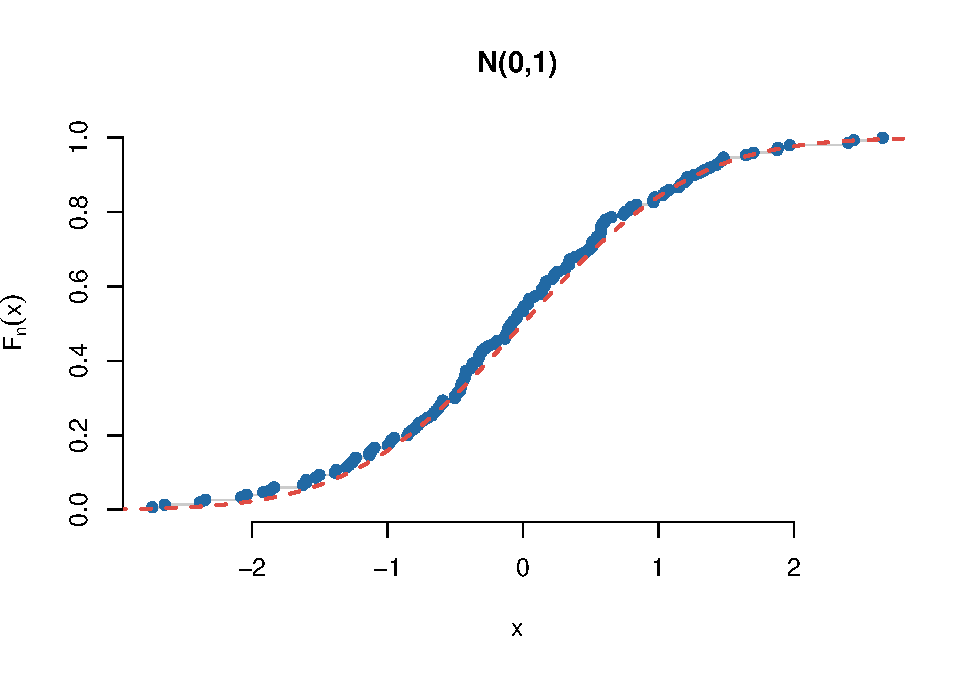
\includegraphics[width=0.7\linewidth]{Lab5_files/figure-latex/unnamed-chunk-4-1} \end{center}

și proprietatea de normalitate (TLC)

\begin{center}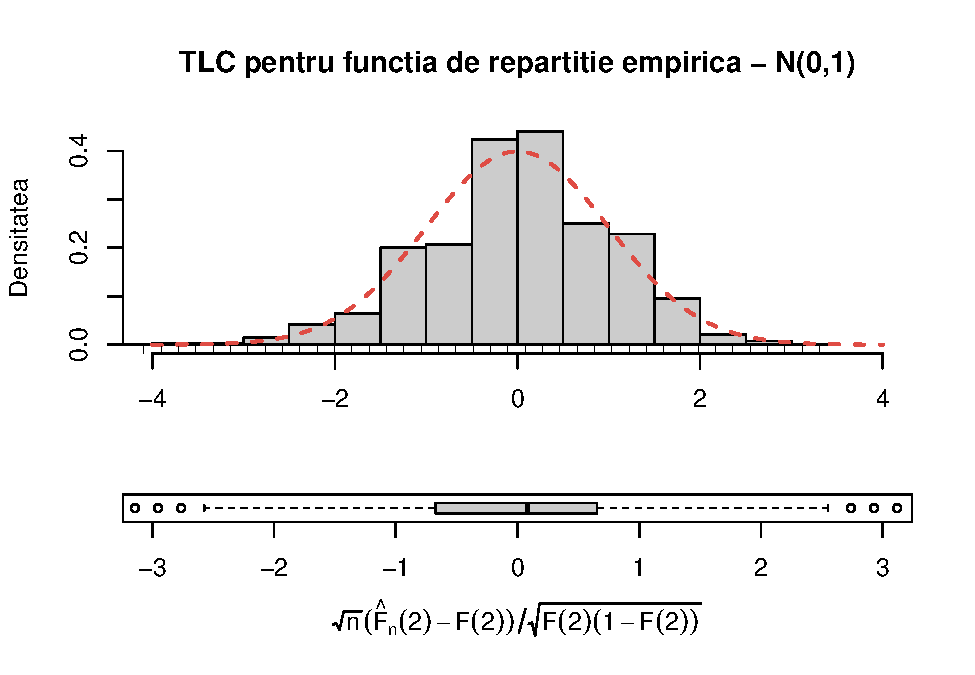
\includegraphics[width=0.7\linewidth]{Lab5_files/figure-latex/unnamed-chunk-5-1} \end{center}

Pentru repartiția \(\mathcal{E}(3)\) avem

\begin{center}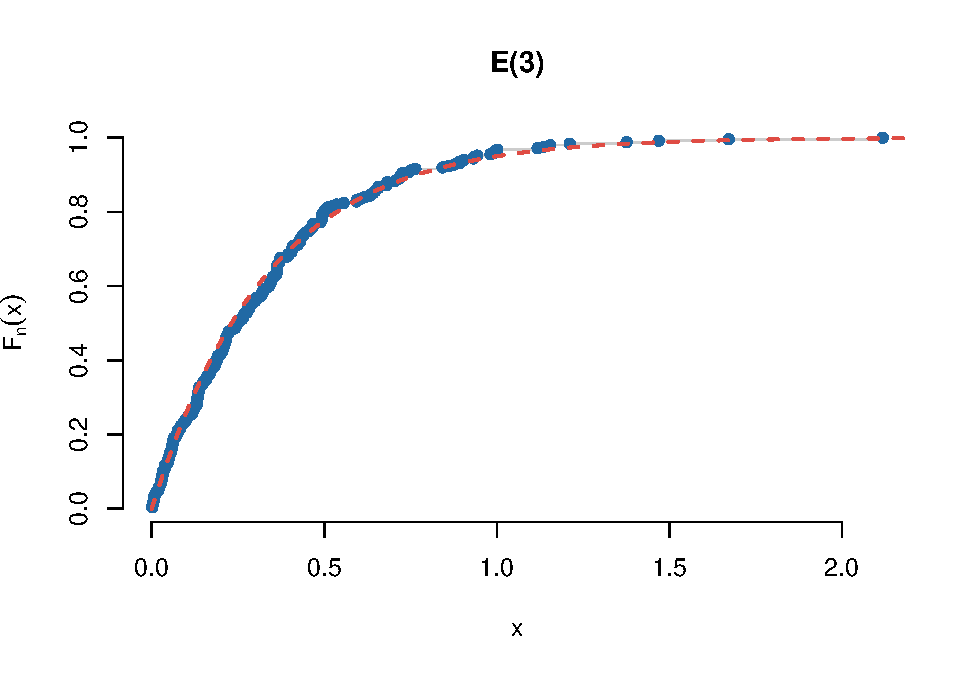
\includegraphics[width=0.7\linewidth]{Lab5_files/figure-latex/unnamed-chunk-6-1} \end{center}

și rezultatul de normalitate asimptotică

\begin{center}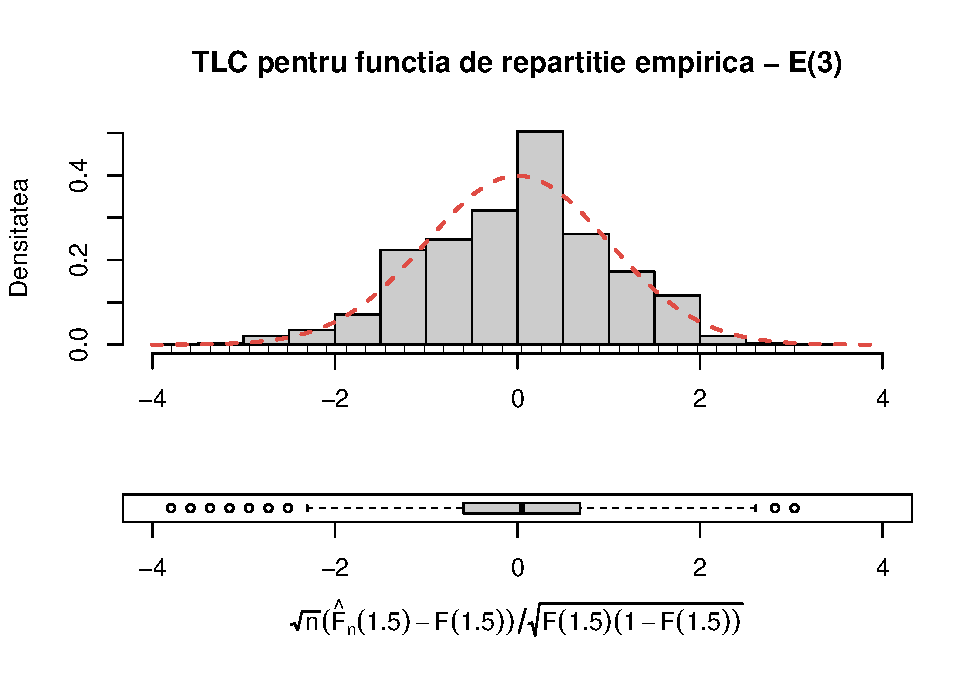
\includegraphics[width=0.7\linewidth]{Lab5_files/figure-latex/unnamed-chunk-7-1} \end{center}

Conform rezultatului anterior putem spune că \(\hat{F}_n(x)\) este un
estimator \emph{rezonabil} pentru funcția de repartiție \(F(x)\) dat
fiind o valoare \(x\in\mathbb{R}\) fixată. Întrebarea care se pune este
dacă \(\hat{F}_n(x)\) este un estimator \emph{rezonabil} pentru întreaga
funcție de repartiție \(F(x)\) ? Răspunsul la această întrebare este dat
de \emph{Teorema Glivenko-Cantelli}\footnote{Pentru o demonstrație a
  acestei teoreme se poate consulta, spre exemplu, cartea lui Sidney
  Resnick \emph{A probability path}, Springer, 1998 (pag 224)} de mai
jos:

\begin{rmdinsight}
\textbf{Teorema Glivenko-Cantelli}. Fie \((X_n)_n\) un șir de variabile
aleatoare independent și identic repartizate, cu funcția de repartiție
comună \(F\). Atunci are loc

\[
  \sup_{x\in\mathbb{R}}\left|\hat{F}_n(x) - F(x)\right| \overset{a.s.}{\underset{n\to\infty}\longrightarrow} 0.
\]
\end{rmdinsight}

\section{Cuantile empirice}\label{cuantile-empirice}

Reamintim că dată fiind o funcție de repartiție \(F\), funcția
\emph{cuantilă} (inversa generalizată) asociată lui \(F\),
\(F^{-1}:(0,1)\to\mathbb{R}\) este definită prin

\[
  F^{-1}(u) = \inf\{x\in\mathbb{R}\,|\,F(x)\geq u\}, \quad \forall u\in(0,1)
\] unde folosim convențiile \(\inf\mathbb{R} = -\infty\) și
\(\inf\emptyset = +\infty\).

\begin{rmdinsight}
Funcția cuantilă \(F^{-1}\) verifică următoarele proprietăți:

\begin{enumerate}
\def\labelenumi{\arabic{enumi})}
\tightlist
\item
  Valoarea în \(0\): \(F^{-1}(0) = -\infty\)
\item
  Monotonie: \(F^{-1}\) este crescătoare
\item
  Continuitate: \(F^{-1}\) este continuă la stânga
\item
  Echivalență: pentru \(\forall u\in[0,1]\) avem
  \(F(x)\geq u \iff x\geq F^{-1}(u)\)
\item
  Inversabilitate: \(\forall u\in[0,1]\) avem
  \((F\circ F^{-1})(u)\geq u\). În plus

  \begin{enumerate}
  \def\labelenumii{\alph{enumii})}
  \tightlist
  \item
    dacă \(F\) este continuă atunci \(F\circ F^{-1} = Id\) dar dacă nu
    este injectivă atunci există \(x_0\) așa încât
    \((F^{-1}\circ F)(x_0)<x_0\)
  \item
    dacă \(F\) este injectivă atunci \(F^{-1}\circ F = Id\) dar dacă nu
    este continuă atunci există \(u_0\) astfel că
    \((F\circ F^{-1})(u_0)>u_0\)
  \end{enumerate}
\end{enumerate}
\end{rmdinsight}

Pentru a exemplifica punctul 5a, putem considera variabila aleatoare
\(X\sim\mathcal{U}[0,1]\) a cărei funcție de repartiție \(F\) este
continuă dar nu injectivă și în plus
\((F^{-1}\circ F)(2) = F^{-1}(1) = 1 < 2\). Pentru punctul 5b să
considerăm variabilele aleatoare \(Y\sim\mathcal{N}(0,1)\) și
\(B\sim\mathcal{B}(0.5)\) independente și să definim \(X = BY\). Atunci
funcția de repartiție a lui \(X\) verifică \(F(0-) = \frac{1}{4}\) și
\(F(0) = \frac{3}{4}\), este injectivă dar nu și continuă în \(0\) și în
plus avem \((F\circ F^{-1})(1/2) = F(0) = \frac{3}{4}>\frac{1}{2}\).

Se numește \emph{cuantilă} de ordin \(p\in(0,1)\) (sau \(p\)-cuantilă)
asociată lui \(F\) valoarea

\[
  x_p = F^{-1}(p) = \inf\{x\in\mathbb{R}\,|\,F(x)\geq p\}.
\]

Cuantila de ordin \(0.5\), \(x_{\frac{1}{2}}\) se numește mediana lui
\(F\) și se notează cu \(M\) sau \(Q_2\), iar cuantilele de ordin
\(\frac{1}{4}\) și respectiv \(\frac{3}{4}\) se numesc prima și
respectiv a treia cuartilă și se notează cu \(Q_1\) și respectiv
\(Q_3\).

Fie acum \(X_1,X_2,\ldots,X_n\) un eșantion de talie \(n\) dintr-o
populație a cărei funcție de repartiție este \(F\) și fie \(\hat{F}_n\)
funcția de repartiție empirică asociată. Pentru \(p\in(0,1)\) definim
cuantila empirică de ordin \(p\) și o notăm \(\hat{x}_p = \hat{x}_p(n)\)
valoarea

\[
  \hat{x}_p = \hat{F}_n^{-1}(p) = \inf\{x\in\mathbb{R}\,|\,\hat{F}_n(x)\geq p\}.
\]

Folosind convenția \(X_{(0)}=-\infty\), cunatila empirică de ordin \(p\)
coincide cu una dintre statisticile de ordine:

\[
  \hat{x}_p = X_{(i)} \iff np\leq i< np+1 \iff \hat{x}_p = X_{(\lceil np \rceil)},
\]

unde \(\lceil x \rceil\) reprezintă cea mai mică valoare întreagă mai
mare sau egală cu \(x\).

Are loc următorul rezultat\footnote{O demonstrație a acestui rezultat
  care nu necesită funcții caracteristice se regăsește în articolul lui
  Jan Wretman \emph{A Simple Derivation of the Asymptotic Distribution
  of a Sample Quantile}, Scand. J. Statist., 5(2): 123-124, 1978.}:

\begin{rmdinsight}
Fie \(X_1,X_2,\ldots,X_n\) un eșantion de talie \(n\) dintr-o populație
cu funcția de repartiție \(F\), \(p\in(0,1)\) fixat, \(x_p\) cuantila de
ordin \(p\) asociată lui \(F\) și \(\hat{x}_p(n)\) cuantila empirică de
ordin \(p\). Atunci

\begin{enumerate}
\def\labelenumi{\arabic{enumi})}
\tightlist
\item
  Convergența: dacă \(F\) este strict crescătoare în \(x_p\) are loc
\end{enumerate}

\[
  \hat{x}_p(n) \overset{a.s.}{\underset{n\to\infty}\longrightarrow} x_p
\]

\begin{enumerate}
\def\labelenumi{\arabic{enumi})}
\setcounter{enumi}{1}
\tightlist
\item
  Normalitatea asiptotică: dacă \(F\) este derivabilă în \(x_p\) cu
  derivata \(f(x_p)>0\), atunci
\end{enumerate}

\[
  \sqrt{n}(\hat{x}_p(n) - x_p)\overset{d}{\underset{n\to\infty}\longrightarrow}\mathcal{N}\left(0,\frac{p(1-p)}{f(x_p)^2}\right).
\]
\end{rmdinsight}

Pentru a ilustra importanța condiției de la primul punct (\(F\) este
strict crescătoare în \(x_p\)) să considerăm
\(X\sim\mathcal{B}(\frac{1}{2})\). Atunci mediana sa este
\(x_{\frac{1}{2}} = 0\) pe când mediana empirică
\(\hat{x}_{\frac{1}{2}}(n)\) va oscila mereu (dar neregulat) între
valorile \(0\) și \(1\).

\begin{center}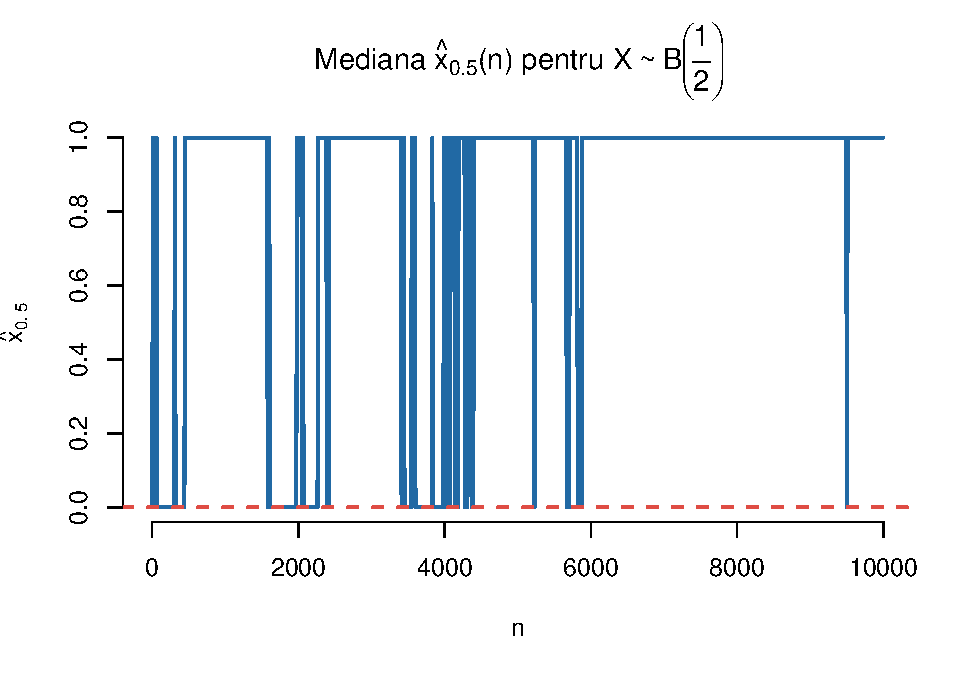
\includegraphics[width=0.7\linewidth]{Lab5_files/figure-latex/unnamed-chunk-11-1} \end{center}

\begin{rmdexercise}
Ilustrați grafic în R proprietatea de convergență și de normalitate
asiptotică (din rezultatul precedent) pentru o populație repartizată
\(\mathcal{N}(0,1)\) și respectiv \(\mathcal{E}(3)\) și pentru
\(p\in\left\{\frac{1}{4}, \frac{1}{2}, \frac{3}{4} \right\}\).
\end{rmdexercise}

În cazul \(\mathcal{N}(0,1)\) avem proprietatea de convergență a
cuantilelor

\begin{center}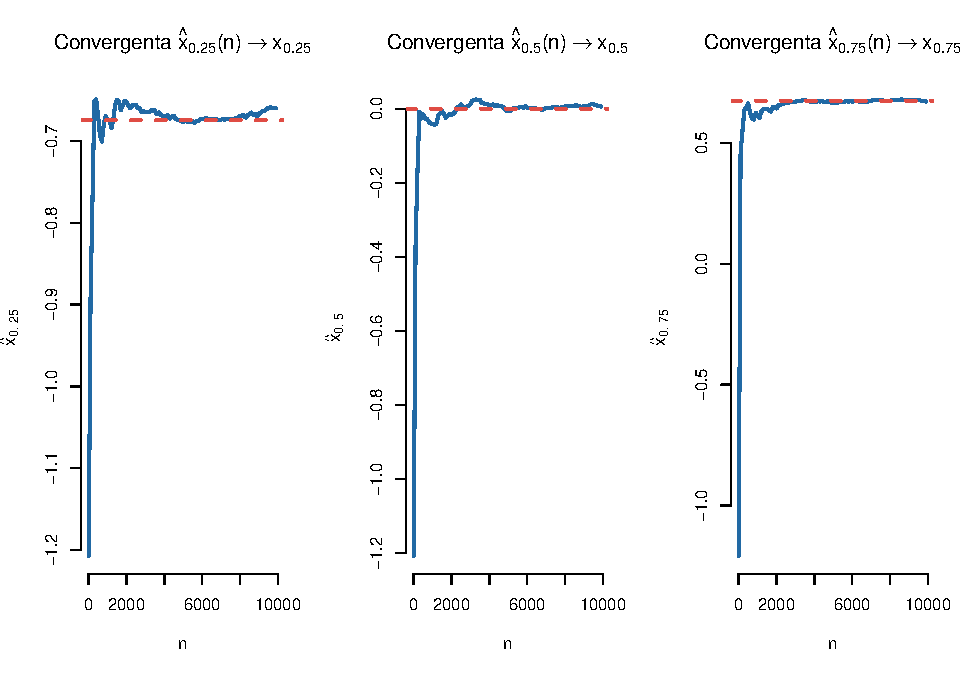
\includegraphics[width=0.7\linewidth]{Lab5_files/figure-latex/unnamed-chunk-13-1} \end{center}

și proprietatea de normalitate asimptotică

\begin{center}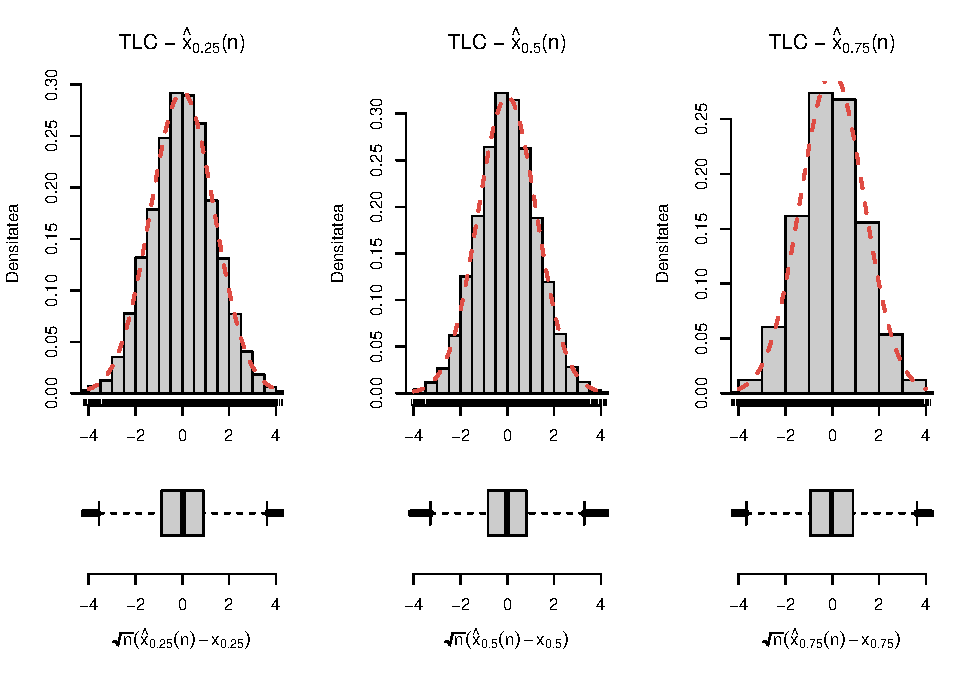
\includegraphics[width=0.8\linewidth]{Lab5_files/figure-latex/unnamed-chunk-14-1} \end{center}

În cazul \(\mathcal{E}(3)\) avem proprietatea de convergență a
cuantilelor

\begin{center}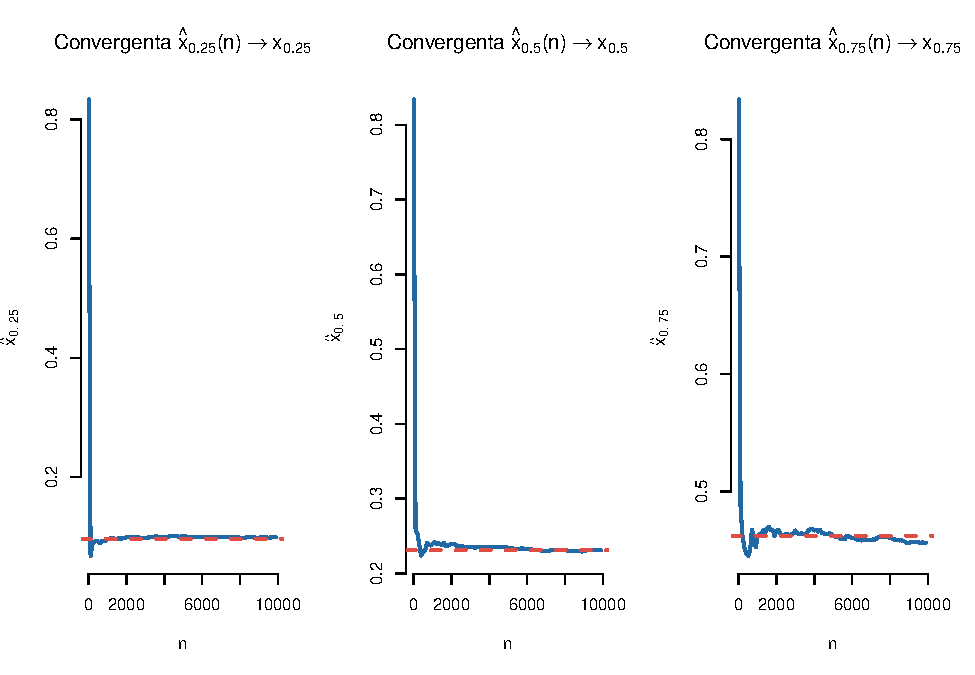
\includegraphics[width=0.7\linewidth]{Lab5_files/figure-latex/unnamed-chunk-15-1} \end{center}

și proprietatea de normalitate asimptotică

\begin{center}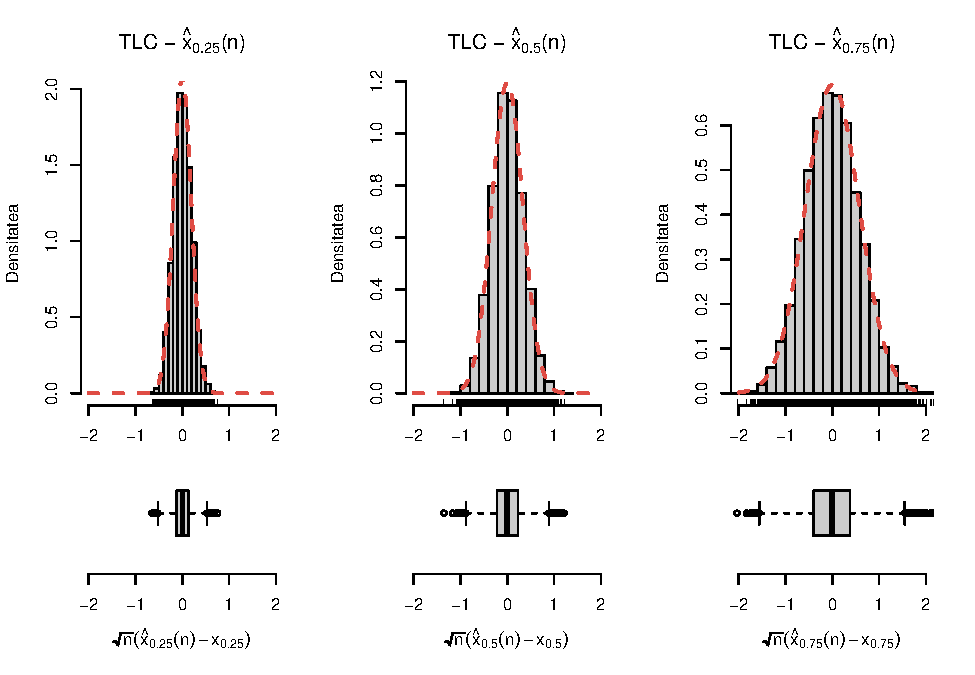
\includegraphics[width=0.8\linewidth]{Lab5_files/figure-latex/unnamed-chunk-16-1} \end{center}

\section{Metoda grafică: Boxplot}\label{metoda-grafica-boxplot}

Una dintre metodele grafice des întâlnite în vizualizarea datelor
(cantitative) unidimensionale este \emph{boxplot}-ul (eng. \emph{box and
whisker plot} - cutia cu mustăți). Această metodă grafică descriptivă
este folosită în principal pentru a investiga forma repartiției
(simetrică sau asimetrică) datelor dar și variabilitatea acestora precum
și pentru detectarea și ilustrarea schimbărilor de locație și variație
între diferitele grupuri de date.

După cum putem vedea și în figura de mai jos, cutia este definită, de la
stânga la dreapta (sau de jos în sus în funcție de cum este reprezentat
boxplot-ul: orizontal sau vertical), de prima cuartilă \(Q_1\) și de a
treia curatilă \(Q_3\) ceea ce înseamnă că \(50\%\) dintre observații se
află în interiorul cutiei. Linia din interiorul cutiei este determinată
de mediană sau a doua cuartilă \(Q_2\).

Mustățile care pornesc de o parte și de alta a cutiei sunt determinate
astfel (vom folosi conveția folosită de John Tukey\footnote{A se
  consulta pag. 40-56 din cartea lui John Tukey \emph{Exploratory data
  analysis}, Addison-Wesley Publishing Company, 1977}): mustața din
stânga este determinată de cea mai mică observație mai mare decât
\(Q_1-1.5 IQR\) iar cea din dreapta de cea mai mare observație din setul
de date mai mică decât \(Q_3+1.5IQR\), unde \(IQR = Q_3-Q_1\) este
distanța dintre cuartile (\emph{interquartile range}).

Valorile observațiilor din setul de date care sunt sau prea mici sau
prea mari se numesc valori aberante (\emph{outliers}) și conform lui
Tukey sunt definite astfel: \emph{valori strict aberante} care se află
la \(3IQR\) deasupra celei de-a treia curtilă \(Q_3\) sau la \(3IQR\)
sub prima cuartilă (\(x<Q_1-3IQR\) sau \(x>Q_3+3IQR\)) și \emph{valori
potențial aberante} care se află la \(1.5IQR\) deasupra celei de-a treia
curtilă \(Q_3\) sau la \(1.5IQR\) sub prima cuartilă (\(x<Q_1-1.5IQR\)
sau \(x>Q_3+1.5IQR\)).

\begin{center}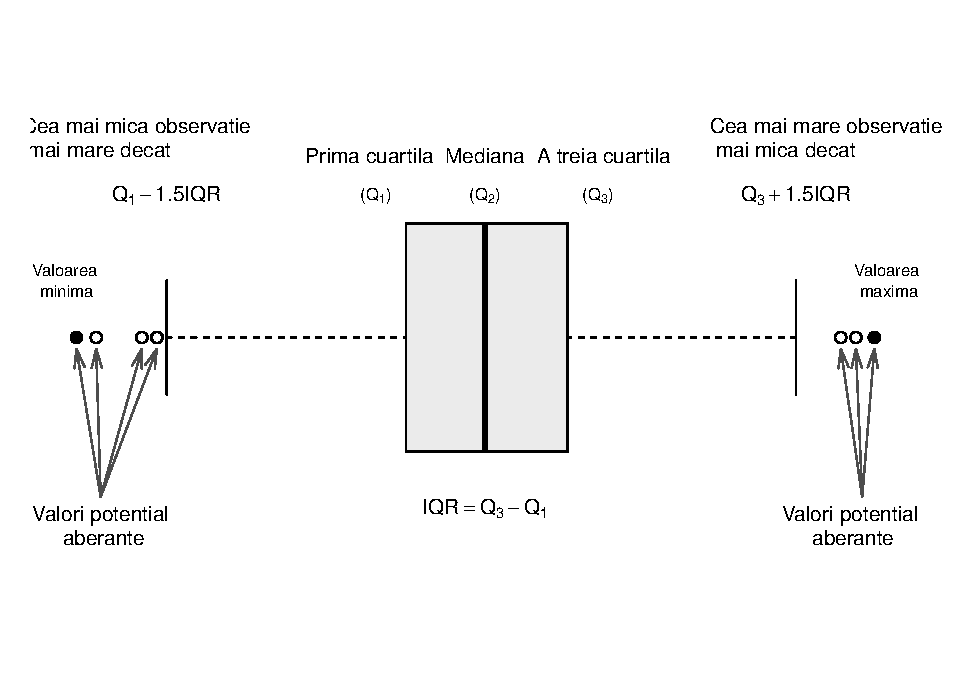
\includegraphics[width=0.7\linewidth]{Lab5_files/figure-latex/unnamed-chunk-17-1} \end{center}

În R metoda grafică boxplot se poate trasa cu ajutorul funcției
\texttt{boxplot()}. Aceasta primește ca argumente sau un vector de
observații numerice \texttt{x} atunci când dorim să ilustrăm repartiția
unei variabile sau o formulă de tipul \texttt{y\textasciitilde{}grup},
unde \texttt{y} este un vector numeric care va fi împărțit în funcție de
variabila discretă \texttt{grup}, atunci când vrem să comparăm aceeași
variabilă numerică în funcție de una discretă (calitatăvă). Pentru mai
multe informații tastați \texttt{?boxplot}.

\begin{rmdexercise}
Considerați setul de date \texttt{mtcars}. Investigați cu ajutorul unui
boxplot cum variază greutatea mașinilor, variabila \texttt{wt}, în
funcție de numărul de cilindrii \texttt{cyl}. Afișați numele mașinilor
care prezintă potențiale valori aberante. Aceeași cerință pentru
perechile \texttt{mpg} - \texttt{cyl}, \texttt{hp} - \texttt{cyl} și
\texttt{hp} - \texttt{am}.
\end{rmdexercise}

\begin{center}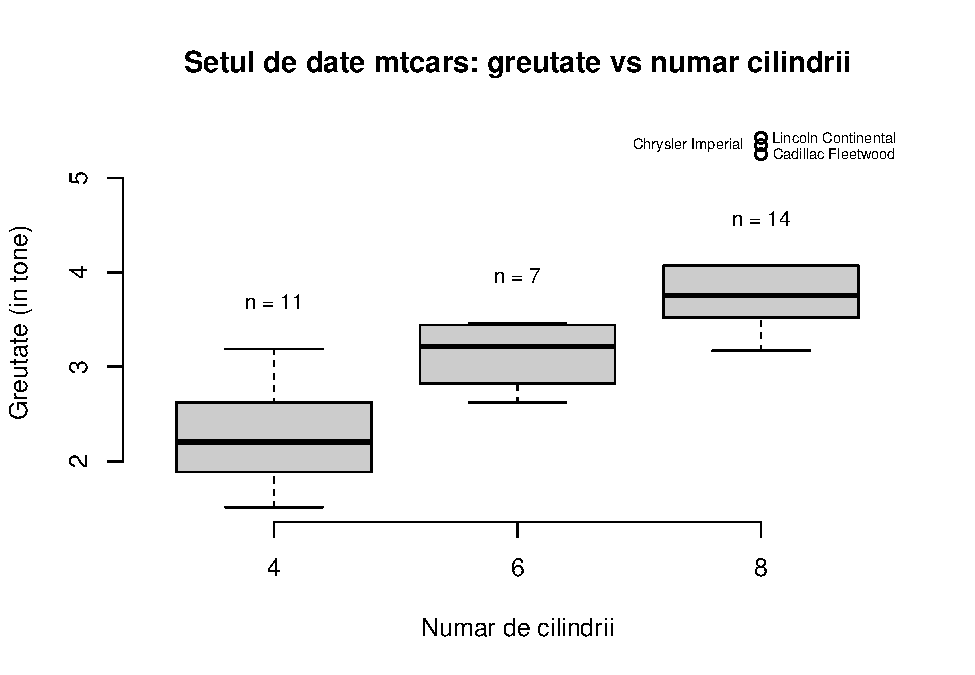
\includegraphics[width=0.7\linewidth]{Lab5_files/figure-latex/unnamed-chunk-19-1} \end{center}

Numele mașinilor care au o greutate potențial aberantă este Cadillac
Fleetwood, Lincoln Continental, Chrysler Imperial.


\end{document}
